%!TEX root = ../../Main.tex

\section{Loading expVIP metadata}\label{loading-expvip-metadata}

This tutorial covers the shell scripts that can be used to load the
metadata with the graphical interface, with screenshots, and the rake
task, to be run in the command line, if you are more comfortable in the
terminal. The assumption is that expVIP is located in
\lstinline!~/expvip-web/!

\subsection{Loading \texttt{factor file}}\label{loading-factor-file}

The first thing to do is to setup the available factors. The
\lstinline!factor file! is a text file, where each field is separated by
tabs. A header is necessary on each column. The headers are the
following:

\begin{itemize}
\itemsep1pt\parskip0pt\parsep0pt
\item
  \textbf{factor}: The name of the factor to group. These must match
  those used in the metadata file (see below).
\item
  \textbf{order}: Default display order in the graphical interface.
\item
  \textbf{name}: The long name of the grouped factor. These must match
  those used in the metadata file (see below).
\item
  \textbf{short}: Short name of the grouped factor. This is used in the
  graphical interface when many factors are displayed.
\end{itemize}

\subsubsection{\texttt{factor file}
example:}\label{factor-file-example}

\begin{lstlisting}
factors order   name    short
Age 1   7 days  7d
Age 2   seedling stage  see
Age 3   14 days 14d
Age 4   three leaf stage    3_lea
Age 5   24 days 24d
Age 6   tillering stage till
Age 7   fifth leaf stage    5_lea
Age 8   1 cm spike  1_sp
Age 9   two nodes detectable    2_no
Age 10  flag leaf stage f_lea
Age 11  anthesis    anth
Age 12  2 dpa   2dpa
Age 13  4 dpa   4dpa
High level age  1   seedling    see
High level age  2   vegetative  veg
High level age  3   reproductive    repr
High level stress-disease   1   none    none
High level stress-disease   2   disease dis
High level stress-disease   3   abiotic abio
High level stress-disease   4   transgenic  trans
High level tissue   1   spike   spike
High level tissue   2   grain   grain
...
\end{lstlisting}

\subsubsection{Wizard to load factors}\label{wizard-to-load-factors}

\begin{enumerate}
\def\labelenumi{\arabic{enumi}.}
\itemsep1pt\parskip0pt\parsep0pt
\item
  Double click in \lstinline!load_factors.sh! in the desktop
  \\ 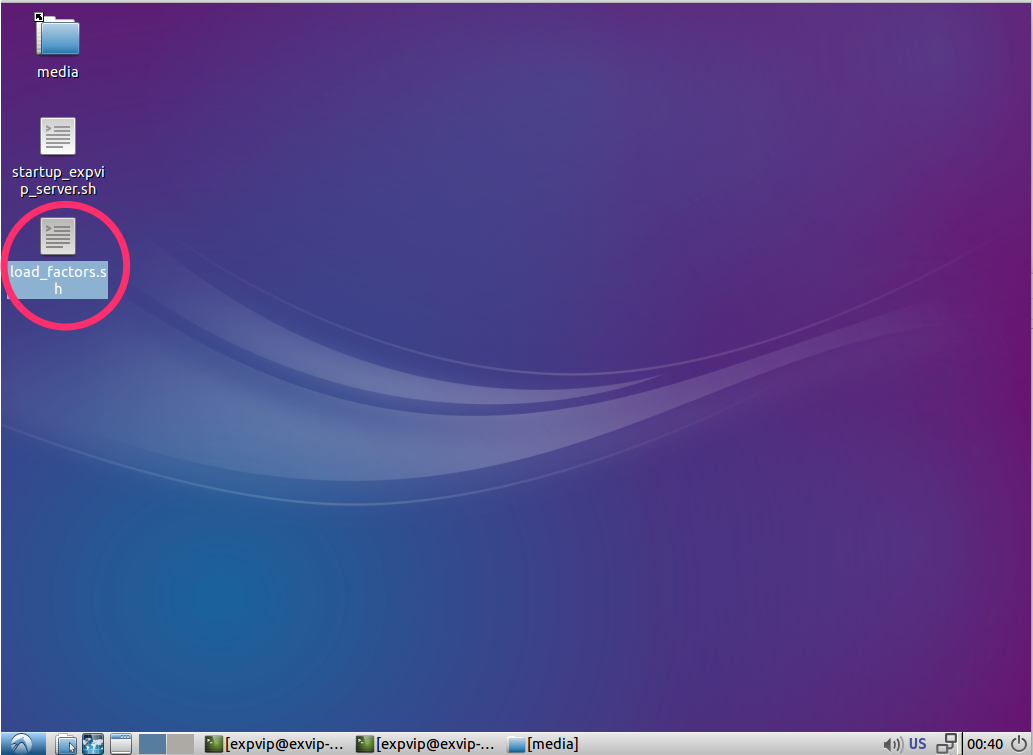
\includegraphics[width=0.75\textwidth]{expVIP/tutorial/images/LoadFactors01.png}
\item
  When prompted, run execute in terminal
  \\ 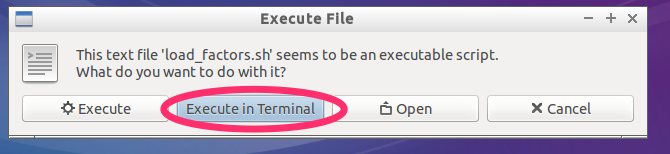
\includegraphics[width=0.75\textwidth]{expVIP/tutorial/images/LoadFactors02.png}
\item
  By default, the script goes to \lstinline!/media!, which is the folder
  containing the \lstinline!shared folders! that we have setup in the
  \url{LoadingVM} step. \\ 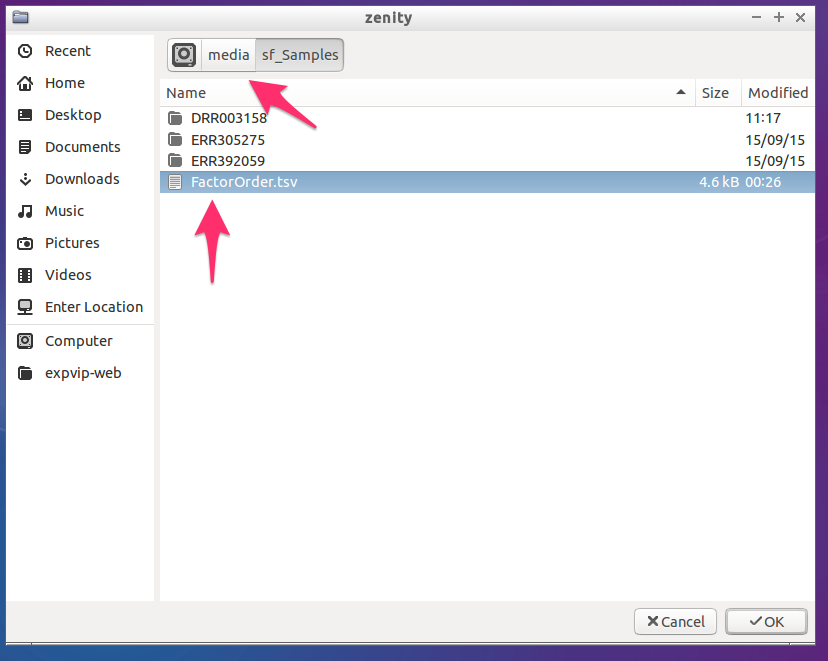
\includegraphics[width=0.75\textwidth]{expVIP/tutorial/images/LoadFactors03.png}
\item
  If the factors are loaded correctly, a pop up window will notify about
  it \\ 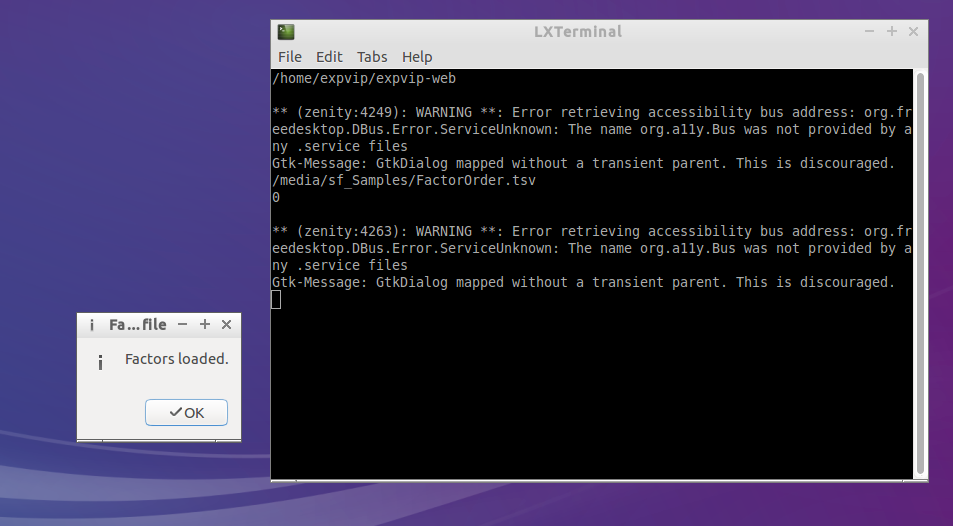
\includegraphics[width=0.75\textwidth]{expVIP/tutorial/images/LoadFactors04.png}
\item
  If there was an error loading the factors, a message will notify about
  it. The error log may give a hint of what went wrong, but if you can't
  figure out send a screenshot of the terminal to the developers.
  \\ 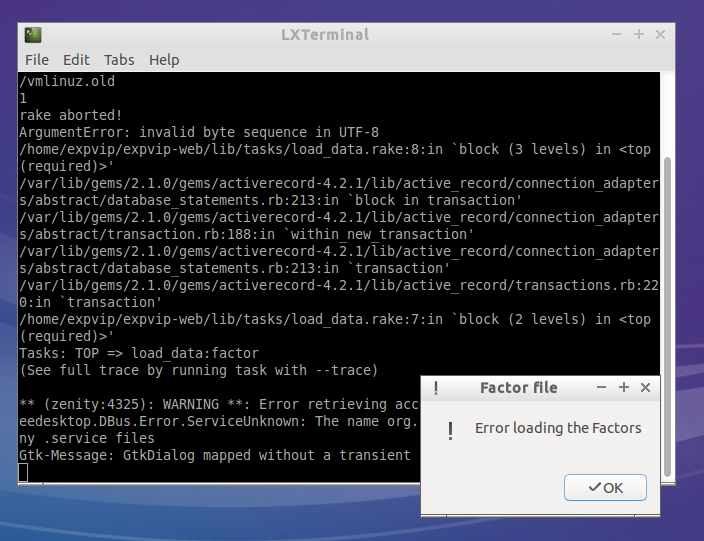
\includegraphics[width=0.75\textwidth]{expVIP/tutorial/images/LoadFactors05.png}
\end{enumerate}

\subsubsection{Rake task}\label{rake-task}

To load the factors, you can run directly the rake task from
\lstinline!~/expvip-web/!.

\begin{lstlisting}
rake load_data:factor[FILE_WITH_FACTORS]; 
\end{lstlisting}

\subsection{Loading metadata}\label{loading-metadata}

The second step is to load the experiment metadata. Currently, a tab
separated file is the input and it \textbf{must} contain the following
columns with the header named exactly as stated:

\begin{itemize}
\itemsep1pt\parskip0pt\parsep0pt
\item
  \textbf{secondary\_study\_accession}: The accession number for
  experiments carried as part of a single study. This is usually the
  high level BioProject or SRA number.
\item
  \textbf{run\_accession}: The accession of the individual run.
\item
  \textbf{scientific\_name}: of the species.
\item
  \textbf{experiment\_title}: A description for the individual RNA-seq
  sample.
\item
  \textbf{study\_title}: A description of the general study.
\item
  \textbf{Variety}
\item
  \textbf{Tissue}
\item
  \textbf{Age}
\item
  \textbf{Stress-disease}
\item
  \textbf{Manuscript}: The DOI of the study.
\item
  \textbf{Group\_for\_averaging} A description of the experiment. This
  must be the same all the replicates in the same study.
\item
  \textbf{Group\_number\_for\_averaging}: A short name for replicated
  experiments.\\
\item
  \textbf{Total reads}: (optional)
\item
  \textbf{Mapped reads}: (optional)
\item
  \textbf{High level variety}: A higher level grouping to get summarised
  data of the factors.
\item
  \textbf{High level tissue}
\item
  \textbf{High level age}
\item
  \textbf{High level stress-disease}
\end{itemize}

\subsubsection{Important points}\label{important-points}

\begin{itemize}
\itemsep1pt\parskip0pt\parsep0pt
\item
  \lstinline!Variety!, \lstinline!Tissue!, \lstinline!Age!,
  \lstinline!Stress-disease!, and their corresponding
  \lstinline!High level! factors must be exactly the same as in the
  columns \lstinline!factor! and \lstinline!name! from the
  \lstinline!factor file! (see above).
\item
  The graphical interface will group samples based on these factors.
  Therefore these can be defined based on the user needs. For example
  the factor \lstinline!High level tissue! will include tissue types
  such as \lstinline!grain!, \lstinline!roots!, \lstinline!spike! and
  \lstinline!leaves/shoots!. Within each of these tissue types, a more
  detailed description can be included under the \lstinline!Tissue!
  heading. For example: \lstinline!starchy endosperm!,
  \lstinline!seed coat!, \lstinline!transfer cells!, etc. RNA-seq
  samples which share factor names in common will be displayed as groups
  in the visual interface.
\item
  If \lstinline!Mapped reads! and \lstinline!Total reads! are missing,
  you need to run \lstinline!kallisto! mapping from the \lstinline!rake!
  task.
\end{itemize}

\subsubsection{Using the graphical
interface}\label{using-the-graphical-interface}

The process is similar to loading the factors. However, the metadata
file is selected.

\begin{enumerate}
\def\labelenumi{\arabic{enumi}.}
\itemsep1pt\parskip0pt\parsep0pt
\item
  Double click on the \lstinline!load_metadata.sh! icon in the desktop
  \\ 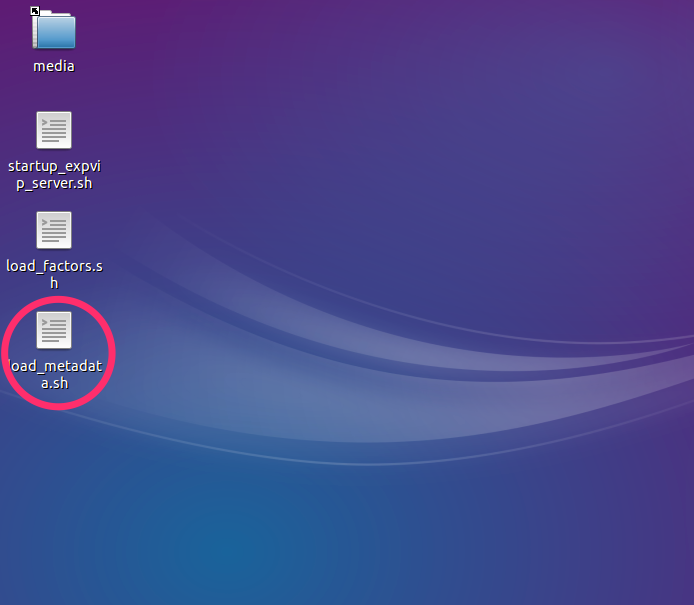
\includegraphics[width=0.75\textwidth]{expVIP/tutorial/images/LoadMetadata01.png}
\item
  Choose execute in terminal \\ 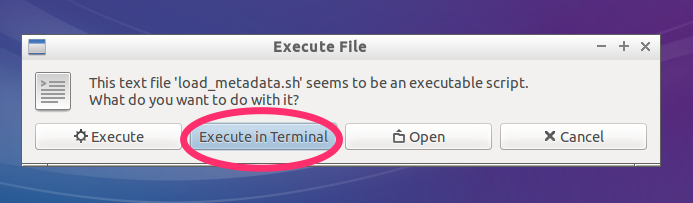
\includegraphics[width=0.75\textwidth]{expVIP/tutorial/images/LoadMetadata02.png}
\item
  Select the metadata file \\ 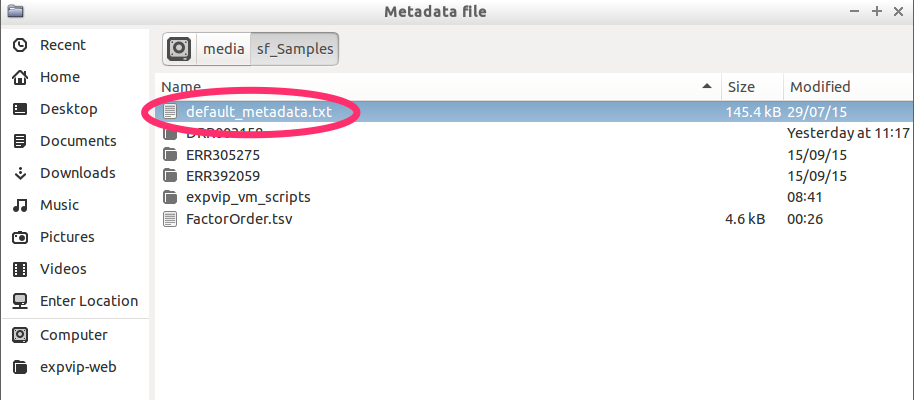
\includegraphics[width=0.75\textwidth]{expVIP/tutorial/images/LoadMetadata03.png}
\end{enumerate}

\subsubsection{Rake task}\label{rake-task-1}

\begin{lstlisting}[language=sh]
rake load_data:metadata[FILE_WITH_THE_METADATA]
\end{lstlisting}

\subsection{Loading the gene sets}\label{loading-the-gene-sets}

Before loading the actual expression data or running kallisto, it is
necessary to load the gene models. Currently, only the fasta file with
the cdna from Ensembl is supported. The fasta header should contain the
following fields, besides the gene name (first string in the header).

\begin{itemize}
\itemsep1pt\parskip0pt\parsep0pt
\item
  \textbf{cdna}
\item
  \textbf{chromosome} or \textbf{scaffold} are converted to position
\item
  \textbf{gene}
\item
  \textbf{transcript}
\item
  \textbf{description} a free text, in quotes. Any other field with
  quotes may fail in the load.
\end{itemize}

Besides the fasta file, it is necessary to give a name to the gene set.
For this tutorial, the \lstinline!gene_set! will be
\lstinline!IWGSC2.26!

\subsubsection{Example fasta file}\label{example-fasta-file}

\begin{code}
>Traes_5BL_3FC5BA305.1 cdna:novel scaffold:IWGSC2:IWGSC_CSS_5BL_scaff_1082268:5:199:-1 gene:Traes_5BL_3FC5BA305 transcript:Traes_5BL_3FC5BA305.1
TGCTGCTGCTAGGCTTGAAGAGGTTGCTGGCAAGCTCCAGTCTGCTCGGCAGCTCATTCA
GAGGGGCTGTGAGGAGTGCCCCAAGAACGAGGATGTTTGGTTCGAGGCATGCCGGTTGGC
TAGCCCAGATGAGTCAAAGGCAGTAATTGCCAGGGGTGTGAAGGCAATTCCCAACTCTGT
GAAGCTGTGGCTGCA
>Traes_6BL_9BB648D51.1 cdna:novel scaffold:IWGSC2:IWGSC_CSS_6BL_scaff_430516:302:1741:-1 gene:Traes_6BL_9BB648D51 transcript:Traes_6BL_9BB648D51.1
TCCCTATCTGTTTCCTTGGCAGCTCCCTGATCCAATCGATCCATCAGGGCTCGACTAACT
TCTTCCAGCGCCTCTTCAGCGCGGGAGATCTACCAGCGTCGGCGGAGGGGCGTAGGTGCA
GGCGTGCAGCCCAAGTCCGCACCCGGCTCTAGGTTTCTGCTAATCTTCTTCCACCTGTGA
TACGCGCTCCGGGGCTAGGAGCACTCGTTGCCGGCTGCCTCGTGCTCGGAATGGCGGATG
\end{code}

\subsubsection{Graphical interface}\label{graphical-interface}

\begin{enumerate}
\def\labelenumi{\arabic{enumi}.}
\itemsep1pt\parskip0pt\parsep0pt
\item
  Double click on the \lstinline!load_gene_set! script
  \\ 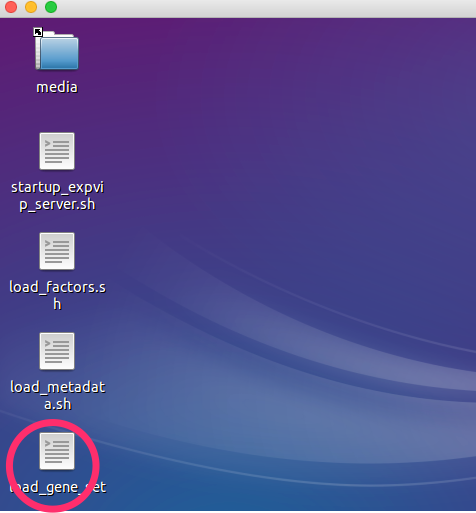
\includegraphics[width=0.75\textwidth]{expVIP/tutorial/images/LoadGeneSet01.png}
\item
  Select \lstinline!Execute in Terminal!
  \\ 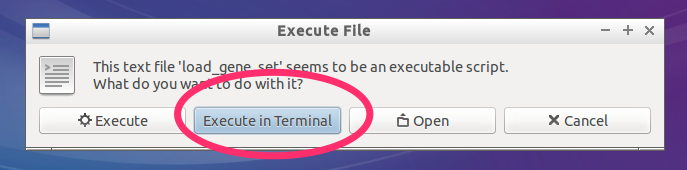
\includegraphics[width=0.75\textwidth]{expVIP/tutorial/images/LoadGeneSet02.png}
\item
  Here you can name the gene set.
  \\ 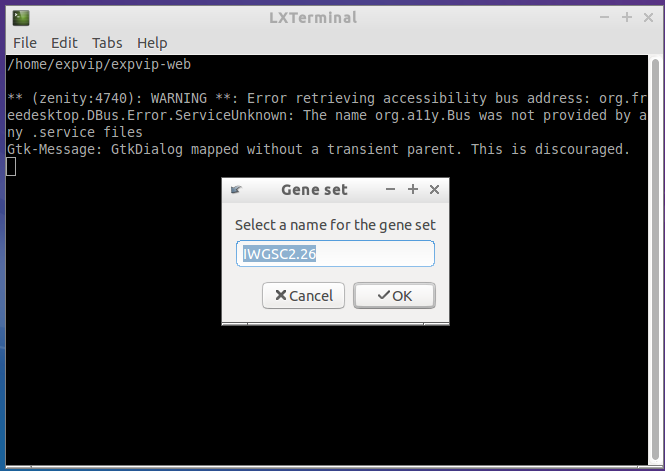
\includegraphics[width=0.75\textwidth]{expVIP/tutorial/images/LoadGeneSet03.png}
\item
  And select the reference file. This may take a few minutes to load.
  \\ 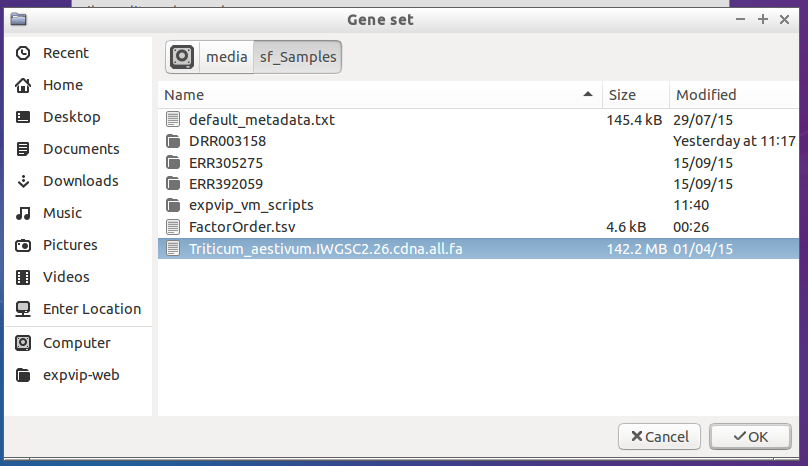
\includegraphics[width=0.75\textwidth]{expVIP/tutorial/images/LoadGeneSet04.png}
\item
  Successfully loaded genes \\ 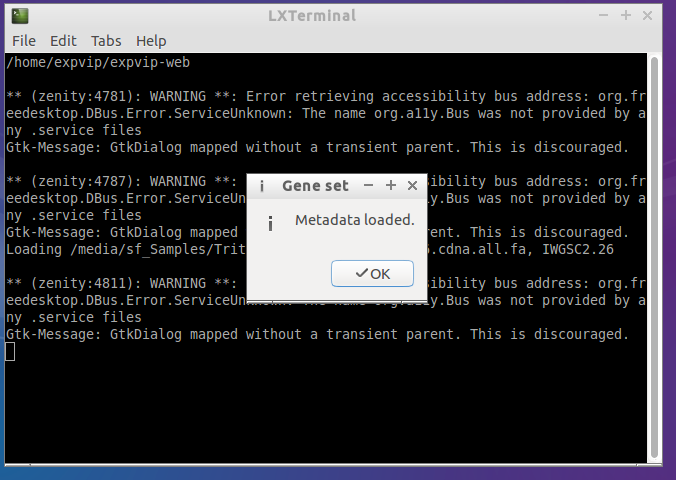
\includegraphics[width=0.75\textwidth]{expVIP/tutorial/images/LoadGeneSet05.png}
\end{enumerate}

\subsubsection{Rake task}\label{rake-task-2}

\begin{code}[language=sh]
rake load_data:ensembl_genes[IWGSC2.26,/Triticum_aestivum.IWGSC2.26.cdna.all.fa]
\end{code}

\subsection{Loading the homoeologues}\label{loading-the-homoeologues}

In order to show the homoeologues, a file with the homoeologies must be
loaded. The file is tab separated with the following format:

\begin{tiny}
\begin{tabular}{llllll}
Gene A & B & D & Group & Genome \\
Traes\_5BS\_0AFC3F795 & Traes\_5BS\_0AFC3F795 & Traes\_5BS\_0AFC3F795 & Traes\_5DS\_C204EBAA9 & 5 & B \\
 Traes\_5DS\_C204EBAA9 & Traes\_5DS\_C204EBAA9 & Traes\_5BS\_0AFC3F795 & Traes\_5DS\_C204EBAA9& 5 & D \\
Traes\_7DL\_82360D4EE1 & Traes\_7DL\_82360D4EE1&Traes\_7DL\_82360D4EE1 & & 7 & D \\
Traes\_2AL\_1368BE0AD &  Traes\_2AL\_1368BE0AD & Traes\_2AL\_1368BE0AD & Traes\_2BL\_CD459994C1 & 2 & A \\ 
\end{tabular}
\end{tiny}

Note that the gene names are not the same as the transcript names, they
correspond to the gene name.

\subsubsection{Generating the file with the homoeologues from Ensembl
compara}\label{generating-the-file-with-the-homoeologues-from-ensembl-compara}

The file can be generated with Ensembl compara, using the following
query:

\begin{code}[language=SQL]
SELECT 
    homology_member.homology_id, cigar_line, perc_cov, perc_id, perc_pos, 
    gene_member.stable_id as genes, 
    gene_member.genome_db_id

FROM 
    homology_member 
INNER JOIN homology USING (homology_id) 
INNER JOIN method_link_species_set USING (method_link_species_set_id) 
INNER JOIN gene_member USING (gene_member_id)
WHERE method_link_species_set.name="T.aes homoeologues";
\end{code}

Then, to format the result of the query (saved as
\lstinline!compara_homology.txt!), you can use the provided script

\begin{lstlisting}[language=sh]
ruby bin/homologyTable.rb compara_homolgy.txt homology.txt homology_counts.txt
\end{lstlisting}

You can get your homoeologies elsewhere, as long as you keep the file
format.

At this point, the homoeologues are called A,B and D. This is going to
change on a future release to allow any chromosome group naming.

\begin{enumerate}
\def\labelenumi{\arabic{enumi}.}
\itemsep1pt\parskip0pt\parsep0pt
\item
  Double click on the \lstinline!load_homoeologues.sh! script
  \\ 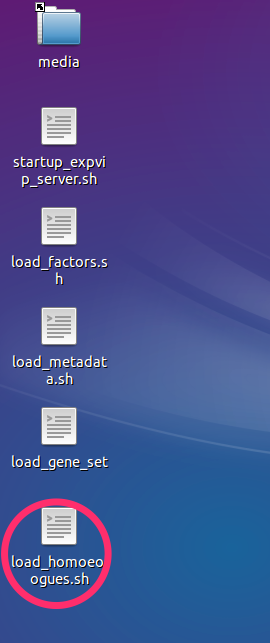
\includegraphics[width=0.75\textwidth]{expVIP/tutorial/images/LoadHom01.png}
\item
  Select \lstinline!Execute in Terminal!
  \\ 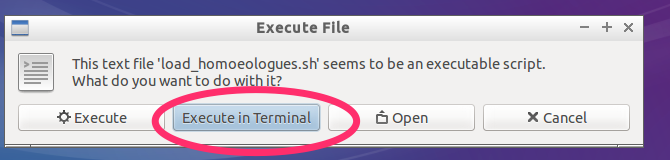
\includegraphics[width=0.75\textwidth]{expVIP/tutorial/images/LoadHom02.png}
\item
  Here you can name the gene set. It must be the same name you added for
  the gene reference. \\ 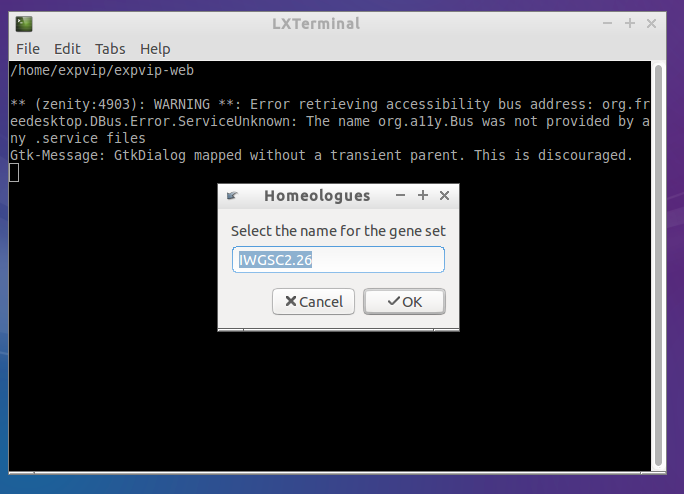
\includegraphics[width=0.75\textwidth]{expVIP/tutorial/images/LoadHom03.png}
\item
  And select the homoeologues file.
  \\ 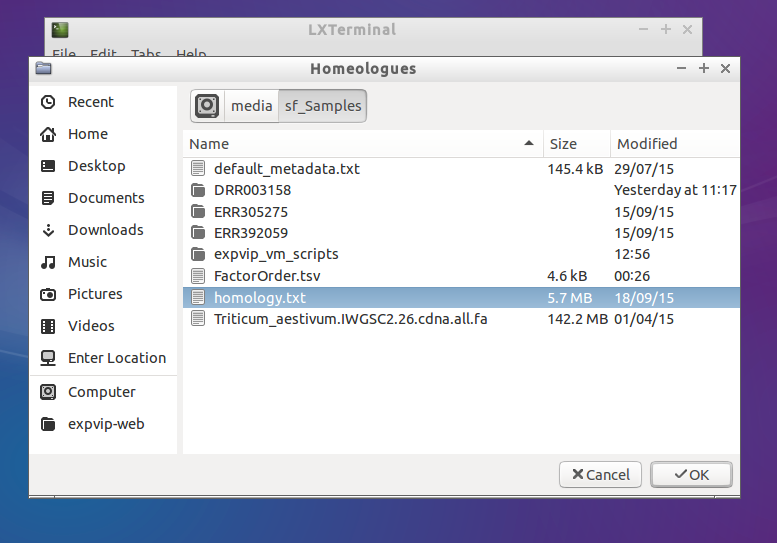
\includegraphics[width=0.75\textwidth]{expVIP/tutorial/images/LoadHom04.png}
\item
  Successfully loaded. At the end of the log you can see which how many
  homoeologies where loaded. \\ 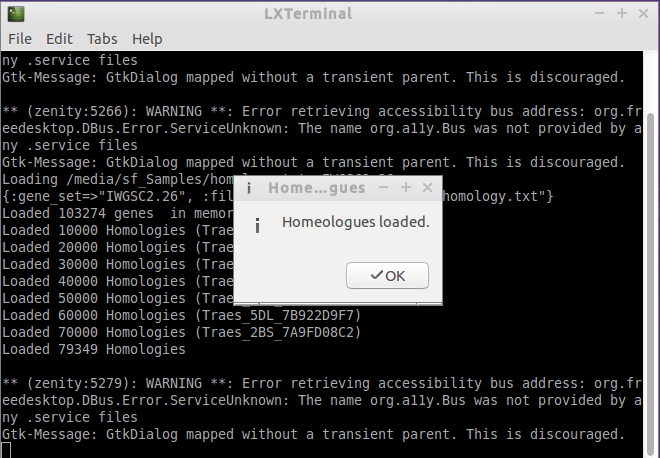
\includegraphics[width=0.75\textwidth]{expVIP/tutorial/images/LoadHom05.png}
\end{enumerate}

\subsubsection{Rake task}\label{rake-task-3}

\begin{lstlisting}[language=sh]
rake load_data:homology[IWGSC2.26,/homology.txt]
\end{lstlisting}

